\section{Einführung}

\textbf{Definition - Financial Management}: Zielgerichtete Beschaffung, Verwendung und Steuerung von unternehmerischem Kapital
\begin{itemize}
	\item \textbf{Finanzierung} = Kapitalbeschaffung
	\item \textbf{Investition} = Kapitalverwendung
	\item Financial Management beschäftigt sich mit \textbf{Liquiditätsplanung, Investitionsstrategie} und \textbf{Finanzierungsstrategie}
	\item Auswirkungen auf Passiv- und Aktivseite der Bilanz
	\item Auswirkungen auf GuV und ihre Interaktion mit der Bilanz
\end{itemize}
\begin{center}
	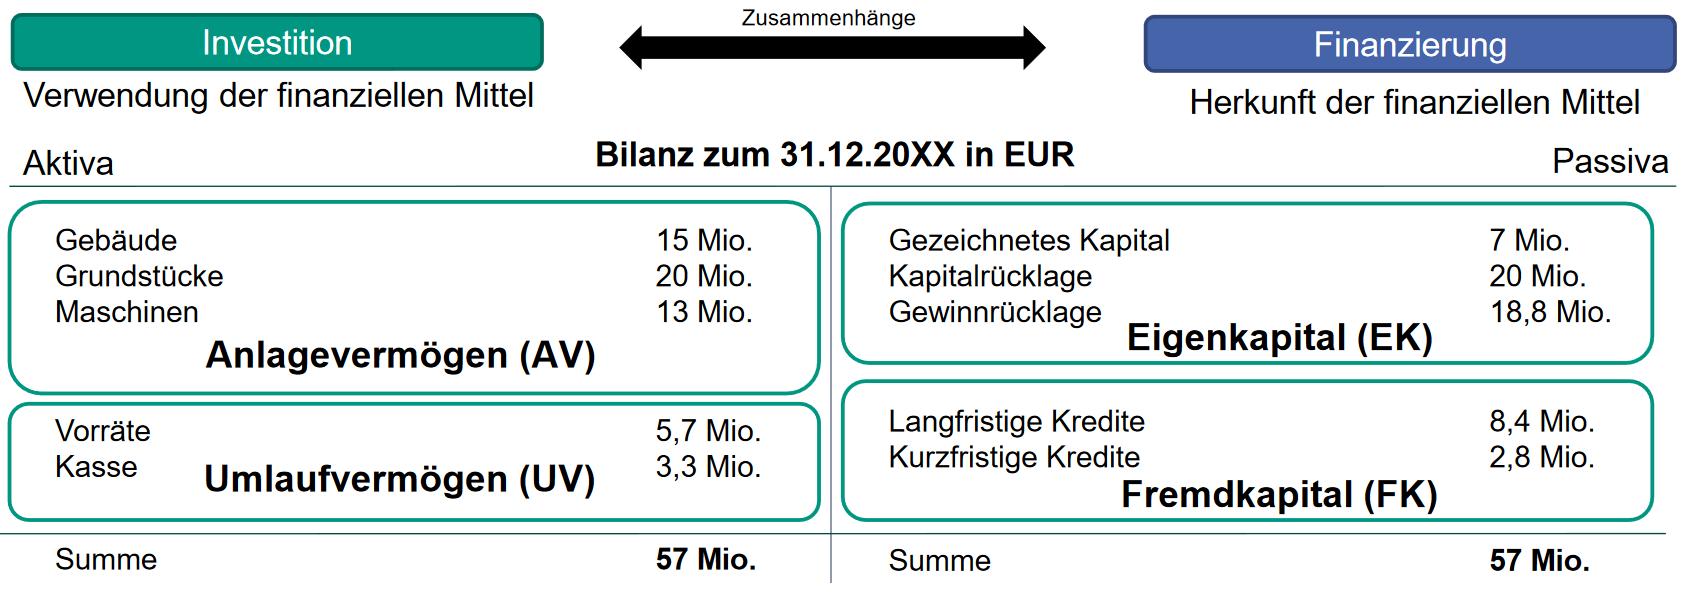
\includegraphics[width=0.8\textwidth]{images/bilanz.png}
\end{center}

\textbf{Ziele des Financial Management}:
\begin{itemize}
	\item Nachhaltige Steigerung des Unternehmenswerts, u.a. durch geeignete Steuerung des Unternehmenswachstums und der Finanzierungskosten
	\item Vermeidung von Illiquidität und Insolvenz
\end{itemize}
\bigskip
\textbf{Finanzielles Gleichgewicht}: Es muss zu jedem Zeitpunkt möglich sein, dass ein Unternehmen seinen Zahlungsverpflichtungen nachkommt: 
$$Z_0+\sum\limits_{n=1}^t E_t\geq\sum\limits_{n=1}^t A_t\qquad\forall t$$

$\rightarrow$ Zahlungsmittelbestand zum Zeitpunkt $t=0$ plus alle Einzahlungen bis zu einem bel. Zeitpunkt $t$ muss mindestens so groß sein wie die Summe aller Auszahlungen bis zum Zeitpunkt $t$

\pagebreak
\textbf{Ermittlung des Zahlungsmittelbestands}:
\begin{center}
	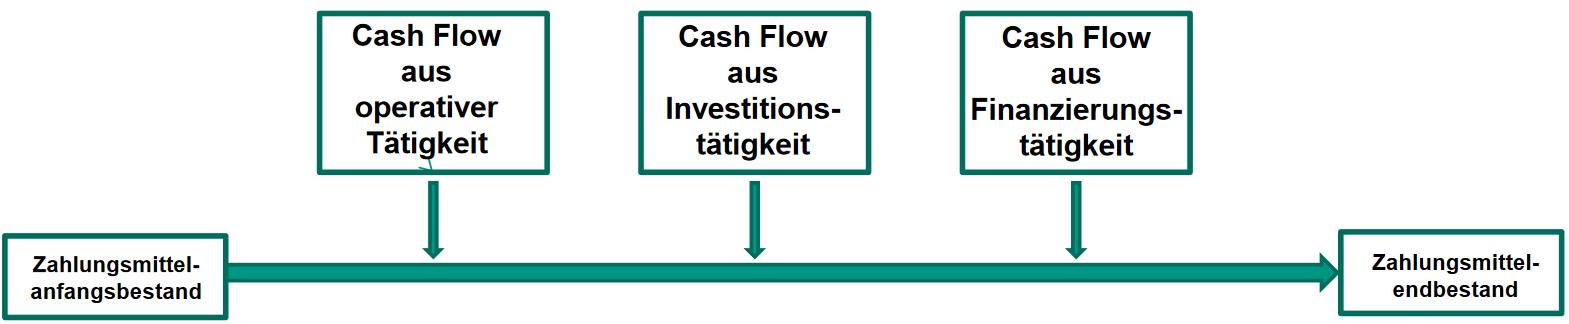
\includegraphics[width=0.8\textwidth]{images/zbestand.png}
\end{center}
\bigskip
\textbf{Planung des Kapitalbedarfs eines Unternehmens}:
\begin{itemize}
	\item \textbf{Liquiditätsplan}: Liquiditätsmäßige Abbildung des operativen Geschäfts $\rightarrow$ kurzfristige Planung der Zahlungsströme
	\item Investitionsplan: Mittel- bis langfristige Abbildung der geplanten Investitionen 
	\item \textbf{Innenfinanzierungsvolumen} = Einzahlungsüberschuss aus gewöhnlicher Geschäftstätigkeit
	\item  Investitionsauszahlungen, die den operativen Cash Flow übersteigen, müssen durch Kapitalzufuhr von außen (EK/FK) finanziert werden
\end{itemize}
\bigskip
\textbf{Formen der Finanzierung}:
\begin{center}
	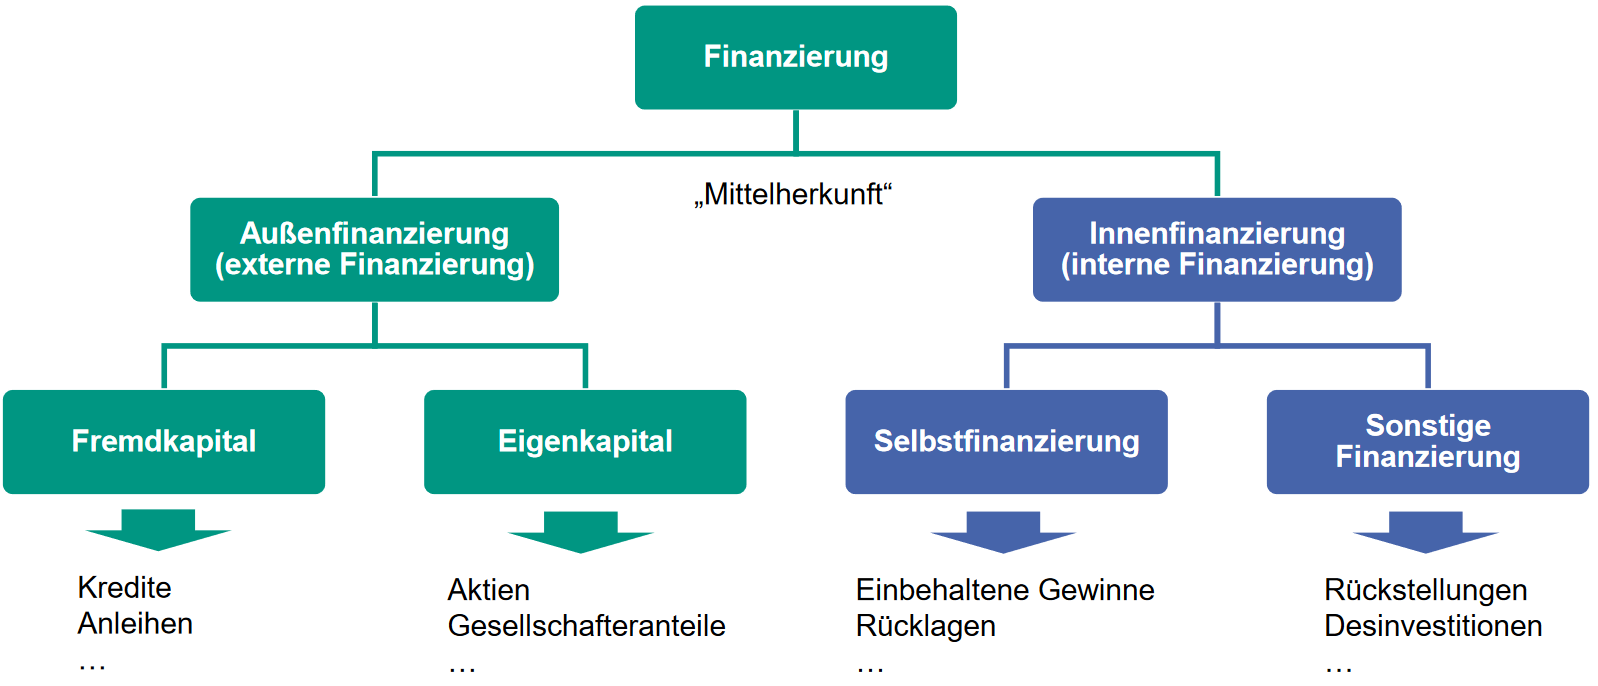
\includegraphics[width=0.8\textwidth]{images/finanzierung.png}
\end{center}
\textbf{Investitions- und Finanzierungsformen je nach Lebensphase eines Unternehmens}:
\begin{itemize}
	\item \textbf{Gründungsphase/Wachstum}: Business Angels, Venture Capital, Eigenkapital (v.a. Einlagen der Gesellschafter), Kredite
	\item \textbf{Wachstum/Reife}: Eigenkapital (Aktien), Fremdkapital (Anleihen, Darlehen)
	\item \textbf{Krise/Insolvenz}: Finanzielle Restrukturierung
\end{itemize}
\bigskip
\textbf{Shareholder Value vs. Stakeholder Value}: Wonach sollten Unternehmen ausgerichtet sein?
\begin{itemize}
	\item \textbf{Shareholder Value}: Ausrichtung der unternehmerischen Tätigkeit an den monetären Interessen der Eigenkapitalgeber (Shareholder)
	\item \textbf{Stakeholder Value}: Fokussierung auf nicht-monetäre Zielsetzungen unterschiedlicher Interessensgruppen (z.B. Management, Mitarbeiter, Lieferanten), Mitbe-rücksichtigung von Reputation und gesellschaftlicher Verantwortung
\end{itemize}